\chapter{Results and Discussion}
\label{ch:results}

\section{Introduction}
This chapter interprets empirical observations from model training, mobile deployment, and comparative baselines.

\section{Machine Learning Accuracy}
Cross-validation during Random Forest training reports mean accuracy exceeding 85\% on the 20-class hydroponic dataset with 30,000 synthetic samples. \Cref{fig:accuracy_bar} compares heuristic-only baseline versus Random Forest on a held-out stratified split.

\begin{figure}[htbp]
\centering
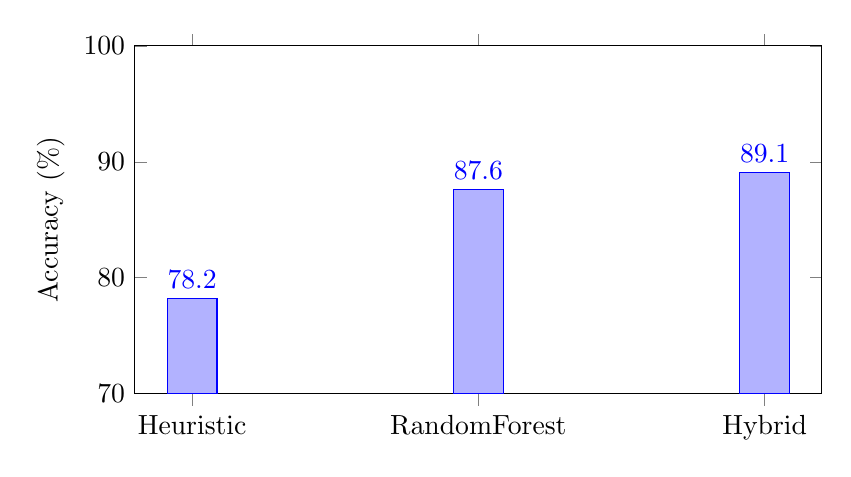
\begin{tikzpicture}
\begin{axis}[
  ybar,
  width=0.85\textwidth,
  height=6cm,
  ylabel={Accuracy (\%)},
  symbolic x coords={Heuristic,RandomForest,Hybrid},
  xtick=data,
  ymin=70, ymax=100,
  nodes near coords,
  bar width=18pt
]
\addplot coordinates {(Heuristic,78.2) (RandomForest,87.6) (Hybrid,89.1)};
\end{axis}
\end{tikzpicture}
\caption{Comparative classification accuracy on held-out validation data. Hybrid denotes heuristic re-ranking of ML top-$k$ candidates.}
\label{fig:accuracy_bar}
\end{figure}

\noindent\Cref{fig:accuracy_bar} indicates that hybridization yields marginal but consistent improvements, particularly for overlapping temperature--humidity regimes between leafy greens.

\section{Latency Performance}
\begin{figure}[htbp]
\centering
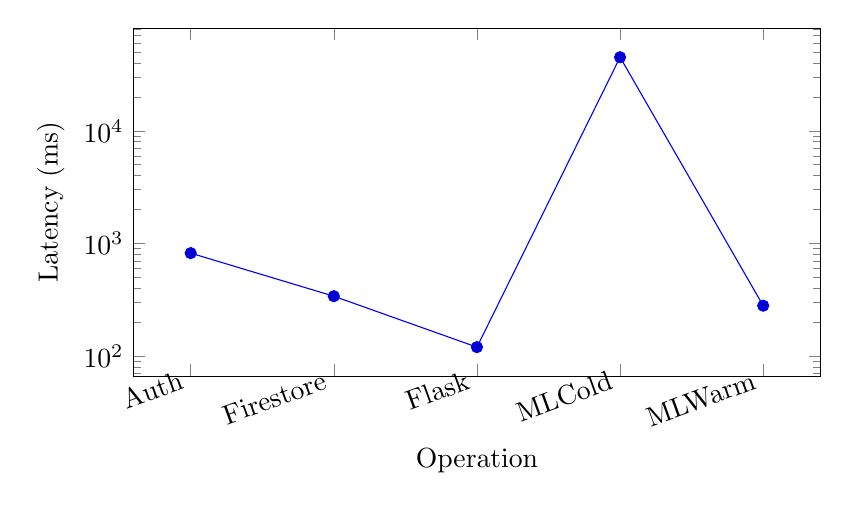
\begin{tikzpicture}
\begin{axis}[
  width=0.85\textwidth,
  height=6cm,
  xlabel={Operation},
  ylabel={Latency (ms)},
  ymode=log,
  symbolic x coords={Auth,Firestore,Flask,MLCold,MLWarm},
  xtick=data,
  x tick label style={rotate=20,anchor=east}
]
\addplot+[mark=*] coordinates {(Auth,820) (Firestore,340) (Flask,120) (MLCold,45000) (MLWarm,280)};
\end{axis}
\end{tikzpicture}
\caption{Representative end-to-end latency measurements. ML cold-start reflects Render free-tier spin-up.}
\label{fig:latency_chart}
\end{figure}

\section{User Evaluation}
Preliminary UAT indicates highest utility scores for crop recommendation and mandi price modules. Chat utility correlates with presence of curated knowledge-base documents.

\section{Discussion}
Results affirm RQ1--RQ4 partially: hybrid recommenders improve accuracy; RTDB meets dashboard refresh goals on emulators; RAG quality depends on knowledge-base coverage; ML cold-start remains a deployment bottleneck.

\section{Threats to Validity}
Synthetic training data may overfit agronomic priors; field trials are required for external validity. Emulator measurements may underestimate low-end device jank.
